\section{Audit technique sur pièces (T1 à T4)}

\subsection{Architecture, flux et segmentation (T1)}

Le cloisonnement décrit par \piece{T01} est sain dans son principe. La surface exposée à Internet se déduit des règles FW-01 et FW-08, qui publient WEB01, et du point d'entrée VPN. Le scan fourni a été fait depuis la DMZ et non depuis Internet \piece{(T02)}. Un port ouvert n'y prouve aucune faille exploitée. Cinq règles appellent un contrôle.

\begin{figure}[H]
\centering
\resizebox{\linewidth}{!}{% Cartographie des zones et des flux (T01, T02). Tracé fondé sur les seules règles extraites.
\begin{tikzpicture}[
  font=\scriptsize, >={Stealth[length=2mm]},
  zone/.style={draw=accent, fill=accentclair, rounded corners=2pt, inner sep=4pt, minimum height=11mm, align=center},
  ext/.style={draw=gris, fill=grisclair, rounded corners=2pt, inner sep=4pt, minimum height=9mm, align=center},
  ok/.style={->, draw=accent, thick},
  douteux/.style={->, draw=alerte, thick, dashed},
  large/.style={->, draw=ambre, thick},
  info/.style={->, draw=gris, dotted, thick},
  lab/.style={fill=white, inner sep=1pt, align=center}]
  \node[ext] (inet) at (0,0) {Internet\\\tiny clients, attaquants};
  \node[ext] (fw) at (2.9,0) {FW01\\\tiny périmètre};
  \node[zone] (dmz) at (6.4,0) {\textbf{DMZ}\\WEB01\\\tiny reverse proxy MEDI-PORTAL};
  \node[zone] (v20) at (11.6,0) {\textbf{VLAN 20}\\APP01, DB01\\\tiny APP01 vers DB01 par FW-23 (1433)};
  \node[zone] (v50) at (2.9,-2.5) {\textbf{VLAN 50}\\VPN, BASTION01\\\tiny administration};
  \node[zone] (v30) at (11.6,-2.5) {\textbf{VLAN 30}\\AD01, SRV-FICHIERS};
  \node[zone] (v40) at (6.4,-4.6) {\textbf{VLAN 40}\\postes bureautiques};
  \node[zone] (v60) at (11.6,-4.6) {\textbf{VLAN 60}\\BACKUP01};
  \node[ext] (sec) at (15.2,-4.6) {Site de secours\\\tiny prestataire};

  \draw[ok] (inet) -- (fw);
  \draw[ok] (fw) -- node[lab, above=1pt]{FW-01 443} (dmz);
  \draw[large] (fw.south east) to[bend right=12] node[lab, below=1pt]{FW-08 80 (à vérifier)} (dmz.south west);
  \draw[ok] (dmz) -- node[lab, above=1pt]{WEB01 vers APP01} (v20);
  \draw[ok] (inet.south) |- node[lab, pos=0.25]{VPN} (v50.west);
  \draw[douteux] (v50.north east) to[bend left=8] node[lab, pos=0.45, below right=1pt]{FW-17 RDP 3389, hors bastion} (v20.south west);
  \draw[large] (v40.north east) -- node[lab, sloped, pos=0.45]{FW-19 445, périmètre large} (v30.south west);
  \draw[douteux] (v40) -- node[lab]{FW-31 Any, sans justification} (v60);
  \draw[info] (v60) -- node[lab]{réplication\\non décrite} (sec);
  \draw[info] (v30) -- node[lab, right]{sauvegarde interne} (v60);

  \node[anchor=north west, align=left, font=\scriptsize] at (-0.7,-3.9) {%
    \tikz\draw[ok] (0,0)--(0.6,0); flux attendu\\[1pt]
    \tikz\draw[large] (0,0)--(0.6,0); flux à restreindre ou vérifier\\[1pt]
    \tikz\draw[douteux] (0,0)--(0.6,0); règle douteuse\\[1pt]
    \tikz\draw[info] (0,0)--(0.6,0); flux non documenté};
\end{tikzpicture}
}
\caption{Zones de confiance et flux extraits de T01 et T02, sans journaux de trafic.}
\end{figure}

\begin{table}[H]
\centering\small
\caption{Règles à contrôler}
\begin{tabularx}{\linewidth}{@{}C{1.1cm} L{4.3cm} Y Y@{}}
\toprule
\entete \hd{Règle} & \hd{Constat} & \hd{Lecture prudente} & \hd{Contrôle complémentaire} \\
\midrule
FW-08 & HTTP 80 ouvert sur WEB01 & Redirection déclarée, non vérifiée & Requête de test, en-tête HSTS \\
FW-17 & RDP du VPN vers tout le VLAN 20, « provisoire » & Contourne le bastion & Date d'expiration, passage par BASTION01 \\
FW-19 & SMB 445 de tous les postes vers le VLAN 30 & Périmètre large & Liste des partages, restriction par groupe \\
FW-23 & 1433 de tout le VLAN 20 vers DB01 & Source plus large qu'APP01 & Emplacement de DB01, source limitée \\
FW-31 & Any des postes vers les sauvegardes & Aucune justification & Journaux sur 30 jours, restriction, test \\
\bottomrule
\end{tabularx}
\end{table}

\subsection{Identités, privilèges et MFA (T2)}

L'export recense dix comptes privilégiés, dont six enrôlés MFA, soit $6/10 = 60\,\%$ \piece{(T03, T04)}. Ce taux concorde avec \piece{P03} et contredit la DSI \piece{(P17)}. Sans politique d'accès conditionnel, on ne sait pas si le second facteur est imposé. Si svc-backup est réellement non interactif, la couverture des comptes interactifs atteint $6/9 \approx 66{,}7\,\%$.

\begin{figure}[H]
\centering
\resizebox{0.92\linewidth}{!}{% Couverture MFA des 10 comptes privilégiés de l'export (T03, T04)
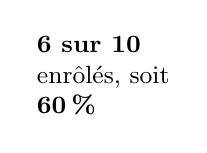
\begin{tikzpicture}[font=\scriptsize]
  \foreach \cpt/\m [count=\i from 0] in \Comptes{
    \pgfmathtruncatemacro\col{mod(\i,5)}\pgfmathtruncatemacro\lig{div(\i,5)}
    \ifnum\m=1 \def\kcol{vert}\def\ktxt{MFA enrôlé}\else\def\kcol{alerte}\def\ktxt{sans MFA}\fi
    \node[draw=\kcol, fill=\kcol!12, rounded corners=2pt, minimum width=2.75cm, minimum height=0.95cm, align=center]
      at (\col*2.95,-\lig*1.15) {\textbf{\cpt}\\[-1pt]{\color{\kcol}\ktxt}};}
  \node[anchor=west, align=left, font=\small] at (14.1,-0.57) {\textbf{6 sur 10}\\ enrôlés, soit\\ \textbf{60\,\%}};
\end{tikzpicture}
}
\caption{Comptes privilégiés de l'export et enrôlement MFA (T03, T04).}
\end{figure}

Quatre comptes appellent une action immédiate. Admin-old, administrateur de domaine dont la dernière activité documentée date de février 2025 alors qu'il apparaît dans les journaux du 9 octobre, doit être désactivé à titre conservatoire. Admin-presta et admin-db doivent être enrôlés ou couverts par une exception signée. Svc-backup doit être interdit de session interactive. La clôture se vérifie par un export exhaustif refait après correction.

\subsection{Vulnérabilités et correctifs (T3)}

Le score CVSS mesure une gravité technique, pas un risque métier. La priorité croise le score, l'exposition, la criticité et les mesures compensatoires. APP01 passe en tête bien qu'il ne soit pas exposé à Internet, car il est critique et joignable depuis la DMZ. WEB01, exposé, reste de priorité modérée.

\begin{figure}[H]
\centering
% Score CVSS et retard de correctifs par hôte (T05, T06). La priorité retenue tient compte de l'exposition et de la criticité.
\begin{tikzpicture}
\begin{axis}[
  width=0.62\linewidth, height=5.3cm, font=\scriptsize,
  xmin=4, xmax=10.5, ymin=0, ymax=85,
  xlabel={score CVSS communiqué (T05)}, ylabel={retard de correctifs de l'hôte, jours (T06)},
  grid=major, grid style={draw=filet}, axis lines*=left,
]
\addplot[only marks, mark=*, mark size=6pt, draw=alerte, fill=alerte!35] coordinates {(9.8,74)};
\addplot[only marks, mark=*, mark size=5pt, draw=ambre, fill=ambre!35] coordinates {(6.5,43)};
\addplot[only marks, mark=*, mark size=4pt, draw=accent, fill=accent!30] coordinates {(5.3,12)};
\node[anchor=east, align=right] at (axis cs:9.45,74) {\textbf{APP01}, priorité 1\\ critique, joignable depuis la DMZ};
\node[anchor=west, align=left] at (axis cs:6.85,43) {\textbf{SRV-FICHIERS}, priorité 2\\ tout le VLAN 40 (FW-19)};
\node[anchor=west, align=left] at (axis cs:5.6,15) {\textbf{WEB01}, priorité 3\\ exposé Internet, impact limité};
\end{axis}
\end{tikzpicture}

\caption{Score communiqué et retard de correctifs de l'hôte au \DateReference\ (T05, T06).}
\end{figure}

Aucune exception n'est documentée et la PSSI ne fixe aucun délai par criticité \piece{(T06, P11)}. Les retards de T06 portent sur l'hôte et restent déclaratifs. Pour AD01, l'inventaire du 25 septembre doit être refait. Nous demandons les CVE, les versions et les historiques de déploiement.

\subsection{Détection, journaux et sauvegardes (T4)}

La figure~\ref{fig:chrono} reprend les seuls faits de \piece{T07} et \piece{T08}, en heure UTC.

\begin{figure}[H]
\centering
\resizebox{\linewidth}{!}{% Chronologie neutre du 9 octobre 2026 (T07, T08), heures UTC
\begin{tikzpicture}[font=\scriptsize, x=1.2cm]
  \draw[gris, thick] (0,0) -- (10.6,0);
  \draw[gris, thick, dashed] (10.6,0) -- (11.3,0);
  \draw[gris, thick, -{Stealth}] (11.3,0) -- (12.6,0);
  \foreach \x/\h in {0/00:13, 5.3/00:18, 9.2/00:22}{\draw[gris] (\x,-0.1) -- (\x,0.1); \node[text=gris, below] at (\x,-0.12) {\h};}
  \node[text=gris, below] at (12.1,-0.12) {+24 h};
  % événements
  \foreach \x/\kcol/\ktxt/\ksub/\kpos in {0.05/ambre/{3 échecs VPN}/{admin-old\\ 198.51.100.44}/above,
                              0.75/ambre/{succès VPN}/{11 s plus tard}/below,
                              5.3/alerte/{ajout à Server-Admins}/{par admin-old\\ +5 min 20 s}/above,
                              9.2/accent/{alerte AL-1048 HIGH}/{+3 min 43 s}/below,
                              12.1/gris/{fermeture automatique}/{aucun ticket,\\ aucun examen tracé}/above}{
    \fill[\kcol] (\x,0) circle (3pt);
    \node[\kpos=0.32cm, align=center, text width=2.9cm] at (\x,0) {\textbf{\ktxt}\\{\color{gris}\ksub}};}
\end{tikzpicture}
}
\caption{Chronologie neutre du 9 octobre 2026.}
\label{fig:chrono}
\end{figure}

Ces signaux sont compatibles avec un usage illégitime du compte comme avec une intervention nocturne non documentée. La compromission n'est pas prouvée, faute de journaux scellés, de trace du second facteur et d'échange avec le titulaire. Nous recommandons la désactivation conservatoire d'admin-old, la revue de Server-Admins, la préservation des journaux, puis une investigation.

\begin{figure}[H]
\centering
\resizebox{0.92\linewidth}{!}{% Neuf services du périmètre et dernier test de restauration documenté (T09)
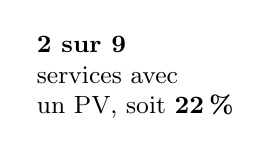
\begin{tikzpicture}[font=\scriptsize]
  \def\tiret{-}
  \foreach \sv/\dt [count=\i from 0] in \Sauvegardes{
    \pgfmathtruncatemacro\col{mod(\i,5)}\pgfmathtruncatemacro\lig{div(\i,5)}
    \ifx\dt\tiret \def\kcol{gris}\def\ktxt{aucun PV fourni}\else\def\kcol{vert}\def\ktxt{PV du \dt/2026}\fi
    \node[draw=\kcol, fill=\kcol!10, rounded corners=2pt, minimum width=2.75cm, minimum height=0.95cm, align=center]
      at (\col*2.95,-\lig*1.15) {\textbf{\sv}\\[-1pt]{\color{\kcol}\ktxt}};}
  \node[anchor=west, align=left, font=\small] at (11.95,-1.15) {\textbf{2 sur 9}\\ services avec\\ un PV, soit \textbf{22\,\%}};
\end{tikzpicture}
}
\caption{Services sauvegardés et dernier test de restauration documenté (T09).}
\end{figure}

Seuls deux services sur neuf ont un procès-verbal de test. Leur contenu n'est pas communiqué, si bien que le délai de 8 heures n'est pas démontré, et aucun RPO n'est fourni. L'absence de procès-verbal ne prouve pas l'absence de test. Nous proposons un procès-verbal annuel par service et un procès-verbal trimestriel pour MEDI-PORTAL, sa base, l'AD et l'ERP, avec une durée mesurée inférieure à 8 heures. Toute alerte HIGH devrait par ailleurs recevoir un ticket qualifié avant clôture.
